% Options for packages loaded elsewhere
\PassOptionsToPackage{unicode}{hyperref}
\PassOptionsToPackage{hyphens}{url}
%
\documentclass[
  12pt,
  a5,margin=2cmpaper,
]{article}
\usepackage{amsmath,amssymb}
\usepackage{iftex}
\ifPDFTeX
  \usepackage[T1]{fontenc}
  \usepackage[utf8]{inputenc}
  \usepackage{textcomp} % provide euro and other symbols
\else % if luatex or xetex
  \usepackage{unicode-math} % this also loads fontspec
  \defaultfontfeatures{Scale=MatchLowercase}
  \defaultfontfeatures[\rmfamily]{Ligatures=TeX,Scale=1}
\fi
\usepackage{lmodern}
\ifPDFTeX\else
  % xetex/luatex font selection
\fi
% Use upquote if available, for straight quotes in verbatim environments
\IfFileExists{upquote.sty}{\usepackage{upquote}}{}
\IfFileExists{microtype.sty}{% use microtype if available
  \usepackage[]{microtype}
  \UseMicrotypeSet[protrusion]{basicmath} % disable protrusion for tt fonts
}{}
\makeatletter
\@ifundefined{KOMAClassName}{% if non-KOMA class
  \IfFileExists{parskip.sty}{%
    \usepackage{parskip}
  }{% else
    \setlength{\parindent}{0pt}
    \setlength{\parskip}{6pt plus 2pt minus 1pt}}
}{% if KOMA class
  \KOMAoptions{parskip=half}}
\makeatother
\usepackage{xcolor}
\usepackage{longtable,booktabs,array}
\usepackage{calc} % for calculating minipage widths
% Correct order of tables after \paragraph or \subparagraph
\usepackage{etoolbox}
\makeatletter
\patchcmd\longtable{\par}{\if@noskipsec\mbox{}\fi\par}{}{}
\makeatother
% Allow footnotes in longtable head/foot
\IfFileExists{footnotehyper.sty}{\usepackage{footnotehyper}}{\usepackage{footnote}}
\makesavenoteenv{longtable}
\usepackage{graphicx}
\makeatletter
\def\maxwidth{\ifdim\Gin@nat@width>\linewidth\linewidth\else\Gin@nat@width\fi}
\def\maxheight{\ifdim\Gin@nat@height>\textheight\textheight\else\Gin@nat@height\fi}
\makeatother
% Scale images if necessary, so that they will not overflow the page
% margins by default, and it is still possible to overwrite the defaults
% using explicit options in \includegraphics[width, height, ...]{}
\setkeys{Gin}{width=\maxwidth,height=\maxheight,keepaspectratio}
% Set default figure placement to htbp
\makeatletter
\def\fps@figure{htbp}
\makeatother
\setlength{\emergencystretch}{3em} % prevent overfull lines
\providecommand{\tightlist}{%
  \setlength{\itemsep}{0pt}\setlength{\parskip}{0pt}}
\setcounter{secnumdepth}{-\maxdimen} % remove section numbering
\newlength{\cslhangindent}
\setlength{\cslhangindent}{1.5em}
\newlength{\csllabelwidth}
\setlength{\csllabelwidth}{3em}
\newlength{\cslentryspacingunit} % times entry-spacing
\setlength{\cslentryspacingunit}{\parskip}
\newenvironment{CSLReferences}[2] % #1 hanging-ident, #2 entry spacing
 {% don't indent paragraphs
  \setlength{\parindent}{0pt}
  % turn on hanging indent if param 1 is 1
  \ifodd #1
  \let\oldpar\par
  \def\par{\hangindent=\cslhangindent\oldpar}
  \fi
  % set entry spacing
  \setlength{\parskip}{#2\cslentryspacingunit}
 }%
 {}
\usepackage{calc}
\newcommand{\CSLBlock}[1]{#1\hfill\break}
\newcommand{\CSLLeftMargin}[1]{\parbox[t]{\csllabelwidth}{#1}}
\newcommand{\CSLRightInline}[1]{\parbox[t]{\linewidth - \csllabelwidth}{#1}\break}
\newcommand{\CSLIndent}[1]{\hspace{\cslhangindent}#1}
\ifLuaTeX
  \usepackage{selnolig}  % disable illegal ligatures
\fi
\IfFileExists{bookmark.sty}{\usepackage{bookmark}}{\usepackage{hyperref}}
\IfFileExists{xurl.sty}{\usepackage{xurl}}{} % add URL line breaks if available
\urlstyle{same}
\hypersetup{
  pdftitle={Streaming convolutional neural networks for end-to-end learning with multi-megapixel images},
  pdfauthor={Hans Pinckaers, Bram van Ginneken, Geert Litjens},
  hidelinks,
  pdfcreator={LaTeX via pandoc}}

\title{Streaming convolutional neural networks for end-to-end learning
with multi-megapixel images}
\author{Hans Pinckaers, Bram van Ginneken, Geert Litjens}
\date{}

\begin{document}
\maketitle

\hypertarget{introduction}{%
\section{Introduction}\label{introduction}}

Convolutional neural networks (CNN) are the current state-of-the-art
machine learning algorithms for many computer vision tasks, such as
classification or segmentation. Ever since Krizhevsky et al.~won
ImageNet\textsuperscript{1} with a CNN\textsuperscript{2} in 2012, these
networks have become deeper\textsuperscript{3} and
wider\textsuperscript{4} to further improve accuracy. Training these
larger networks requires large amounts of computer memory, which
increases exponentially with increasing image size. To avoid
shortcomings in memory, most natural image datasets in computer vision
contain sub-megapixel images: 0.09 megapixel for
ImageNet\textsuperscript{1} and 0.001 megapixel for
CIFAR-10\textsuperscript{5}. In several domains such as remote sensing
or medical imaging, there is a need for training CNNs with
multi-megapixel-sized images -- containing both global contextual and
local textural information -- to obtain accurate models.

Computer memory becomes a limiting factor because the conventional
backpropagation algorithm for optimizing deep neural networks requires
the storage of intermediate activations. Since the size of these
intermediate activations in a convolutional neural network increases
proportionally to the input size of the network, memory quickly fills up
with images of multiple megapixels. As such, only small CNNs could be
trained with these images and state-of-the-art architectures would be
out of reach, even on large computing clusters.

In this paper, we propose a novel method to directly train
state-of-the-art convolutional neural networks using any input image
size end-to-end. This method exploits the locality of most operations in
modern convolutional neural networks by tiling the forward and backward
pass in combination with gradient checkpointing. Gradient checkpointing
is a technique where instead of keeping all intermediate feature maps in
memory to calculate the gradients, we save some specific feature maps
(checkpoints). We recalculate the others by performing partial forward
passes starting from the saved feature maps during backpropagation, once
they are needed for gradient calculation\textsuperscript{6}. We first
empirically established equivalence between our tile-based approach and
an unmodified convolutional neural network on a subset of ImageNet,
ImageNette\textsuperscript{7}. Then we applied this method to two public
datasets: the CAMELYON17 dataset\textsuperscript{8} for metastases
detection in lymph nodes, and the TUPAC16 dataset\textsuperscript{9} for
predicting a proliferation score based on gene expression. In both
cases, task-specific performance increased with larger input image
sizes.

\hypertarget{related-work}{%
\section{Related work}\label{related-work}}

Several authors have suggested approaches to train convolutional neural
networks (CNNs) with large input images while preventing memory
bottlenecks. Their methods can be roughly grouped into three categories:
(A) altering the dataset, (B) altering usage of the dataset, and (C)
altering the network or underlying implementations.

\hypertarget{altering-the-dataset}{%
\subsection{Altering the dataset}\label{altering-the-dataset}}

If images are too large to fit in the memory of the processing unit, we
could downsample the image or divide the image into smaller parts, i.e.,
patches. The latter approach has been prevalent in both remote sensing
and medical imaging\textsuperscript{10,11}. However, both approaches
have significant drawbacks: the former results in a loss of local
details, whereas the latter results in losing global contextual
information.

The common approach of training on patches typically involves creating
labels for every patch, which can be time- and cost-intensive. It is
sometimes not even possible to produce patch-level labels: if a
hypothetical task is to predict whether an aerial image shows a city or
a village, it is impossible to create informative labels for individual
patches only containing several houses.

\hypertarget{altering-usage-of-the-dataset}{%
\subsection{Altering usage of the
dataset}\label{altering-usage-of-the-dataset}}

When we can assume that individual patches contain enough information to
predict the image-level label, the classification can be formalized
under the classic multiple-instance-learning (MIL) paradigm. In MIL,
each image is considered a bag consisting of patches where a positive
bag has at least one positive patch and a negative bag none. In the deep
learning case, a model is trained in a weakly supervised manner on
patches, where the patch with the highest predicted probability is used
for backpropagation\textsuperscript{12,13}. Other approaches involve
taking the average of the patch predictions or a learned weighted
average from low-dimensional patch embeddings\textsuperscript{14--18}.

In this approach, the receptive field of a network is always at most the
size of the patch. The model disregards spatial relationships between
patches, limiting the incorporation of contextual information.

By first learning to decide which regions should be analyzed at a higher
resolution, the problem that a full image cannot be used can also be
circumvented\textsuperscript{19--22}. Since these methods use a
low-resolution version of the image to decide which parts need to be
analyzed at a higher resolution, the low-resolution image needs to have
enough information to localize the area that needs to be classified.
Additionally, for analysis of the selected areas, these methods still
use patch-based analysis with the same caveats as mentioned before.

Another way to utilize datasets with large images is proposed by Tellez
et al.\textsuperscript{23}. To compress the image to a lower-dimensional
space, they proposed unsupervised learning. The model is trained
patch-by-patch to reconstruct the original patch. An intermediate
feature map of the model (i.e., the embedding) can subsequently be used
as a lower-dimensional representation per patch. After training, the
whole image is compressed patch-by-patch. A model is subsequently
trained on these embeddings, having the receptive field of the whole
image while requiring less memory.

Since the compression network is trained by reconstruction, the same
compression network can be used for different tasks. However, this means
that the low-dimensional embedding is not meant for a specific task and
may have compressed away useful information. Our approach involves one
network which learns to compress task-relevant information.

\hypertarget{altering-the-network-or-underlying-implementations}{%
\subsection{Altering the network or underlying
implementations}\label{altering-the-network-or-underlying-implementations}}

The memory bottleneck can also be circumvented with memory-efficient
architectures or memory-efficient implementations of existing
architectures. Recently, Gomez et al.\textsuperscript{24} published a
method to train deep residual neural networks using less memory, termed
the Reversible Residual Network. With these networks, some layer
activations are recomputed from others on demand, reducing the total
memory required. Network architectures can also be altered to utilize
cheaper computational operation, such as depthwise separable
convolutions\textsuperscript{25} or fewer
parameters\textsuperscript{26}. Our method does not require reducing the
number of parameters and works with most types of layers. Another method
to reduce memory usage is to recover intermediate activations by doing
partial forward passes during backpropagation, termed gradient
checkpointing\textsuperscript{6}. This method is similar to our
approach, but the whole activation feature map of some layers still need
to be stored in memory, limiting the use of multi-megapixel images.

Another memory-saving approach is to share memory between tensors with
duplicate or recomputable values\textsuperscript{27,28}, to develop
neural networks with reduced precision using half-precision or mixed
precision\textsuperscript{29}, or to swap data between random access
memory (RAM) and graphics processing unit (GPU)
memory\textsuperscript{30}. These methods are usually insufficient for
training with large multi-megapixel images; our proposed method can work
orthogonally to them.

\hypertarget{methods}{%
\section{Methods}\label{methods}}

To achieve our goal of training CNNs with multi-megapixel images, we
significantly reduce the memory requirements. Memory demand is typically
highest in the first few layers of state-of-the-art CNNs before several
pooling layers are applied because the intermediate activation maps are
large. These activation maps require much less memory in subsequent
layers. We propose to construct these later activations by streaming the
input image through the CNN in a tiled fashion, changing the memory
requirement of the CNN to be based on the size of the tile and not the
input image. This method allows the processing of input images of any
size.

Several problems arise when trying to reconstruct the later activation
map tile-by-tile. Firstly, convolutional layers handle image borders in
different ways, either by padding zeros to perform a ``same''
convolution or by reducing the image size to perform a ``valid''
convolution. Secondly, in tile-based processing, border effects occur at
both the image borders and the tile borders; naive tiling of the input
image would thus result in incomplete activation maps and gradients for
backpropagation. Lastly, intermediate feature maps of the tiles still
need to be stored in memory for backpropagation, which would counteract
the streaming of tiles. We solve these problems by developing a
principled method to calculate the required tile overlap throughout the
network in both the forward and backward pass and by using gradient
checkpointing.

We first explain the reconstruction of the intermediate activation map
in the forward pass in section \protect\hyperlink{forwardpass}{3.1},
then describe the backward pass in section
\protect\hyperlink{backwardpass}{3.2}, elaborate on how to calculate the
tile overlap in section \protect\hyperlink{calculateoverlap}{3.3}, and
finish with the limitations of this method in section
\protect\hyperlink{limitations}{3.4}. See Figure
\protect\hyperlink{figure:streamingSGD}{{[}figure:streamingSGD{]}} for a
graphical representation of the method.

\hypertarget{forwardpass}{%
\subsection{Streaming during the forward pass}\label{forwardpass}}

Without loss of generality, we explain the method in the discrete
one-dimensional case. Let us define \(x \in \mathbb{R}^{N}\) as the
one-dimensional real-valued vector with \(N\) elements. In discrete
one-dimensional space, a ``valid'' convolution\footnote{By convention we
  used the term \emph{convolution} although the mathematical operation
  implemented in most machine learning frameworks (e.g., TensorFlow,
  PyTorch) is a cross-correlation.} (*) with a kernel with \(n\) weights
\(w \in \mathbb{R}^n\), and stride 1, is defined as:

\[\label{eq:1}
(x * w)_k = \sum_{i=0}^{n} w_{i}x_{k+i}\]

where \(k \in \{0,\ldots,f\}\) and \(f=N - n\), for any kernel with
length \(n \leq N\) (for clarity, we will start all indices from 0). Our
goal is to decrease the memory load of an individual convolution by
tiling the input. Following \protect\hyperlink{eq:1}{{[}eq:1{]}}, we can
achieve the same result as \(x * w\), by doing \textbackslash{} two
convolutions on the input: \[\begin{gathered}
a = \{(x * w)_0,\ldots,(x * w)_{f//2}\} 
b = \{(x * w)_{f//2+1},\ldots,(x * w)_f\} \label{eq:3}
\end{gathered}\] where \(//\) denotes a divide and floor operation.

By definition of concatenation (\(\frown\)): \[\label{eq:4}
\{(x * w)_0,\ldots,(x * w)_f\}= a \frown b\]

To ensure that the concatenation of both tiles results in the same
output as for the full vector, we need to increase the size of the
tiles, resulting \(o=n-1\) overlapping values. The values
\(\{ x_0,\ldots,x_{f//2+o} \}\) are required to calculate \(a\), and
\(\{ x_{f//2+1-o},\ldots,x_N \}\) for \(b\).

Since the tiles are smaller than the original vector, these separate
convolutions require less memory when executed in series. By increasing
the number of tiles, memory requirements for individual convolution
operations can be reduced even further.

Without loss of generality, the above can also be extended to multiple
layers in succession including layers with stride \(> 1\) (e.g., strided
convolutions and pooling layers) which are also commonly used in
state-of-the-art networks.

When one applies this tiling strategy naively, no memory benefit is
obtained as each tile's intermediate activation would still be stored in
memory to allow for backpropagation. We use gradient checkpointing to
resolve this: We only store the activations after the concatenation of
the tiles -- where the memory burden is small. This does require
recalculation of all intermediate activations for all tiles during
backpropagation, but again, only has a memory requirement of processing
of a single tile. The trade-off between memory use and re-computation
can be controlled through the selection of the concatenation point in
the network.

From this point onward, the term \emph{streaming} refers to the tiling
of a vector, applying kernel operations, and concatenating the results.

\(o\gets[]\) \(stream\_o\gets\) \texttt{concat}\((o[0..m])\)
\(pred\gets\) \texttt{forward}\((layers[i..n], stream\_o)\)
\(loss\gets\) \texttt{criterion}\((pred)\) \(g\gets\)
\texttt{backward}\((layers[n..i], loss)\) \(filled\gets[]\)

\hypertarget{backwardpass}{%
\subsection{Streaming during backpropagation}\label{backwardpass}}

The backward pass of multiple convolutions can also be calculated by
utilizing the tiles. To start, let us define \(p\) as the output after
streaming. The derivative of a weight in a convolutional kernel is
defined as:

\[% \label{eq:5}
\Delta w_j = \sum_{i=0}^{\lvert p \rvert-1}
\begin{cases}
  \Delta p_i x_{i+j}, & \text{if}\ i - j \geq 0 \text{ and } i - j < \lvert p \rvert \\
%   0 1 2 3 4 = p
%   - - - - -
%       0 1 2 = kernel (j - i \geq 0 \text{and} j - i + n < |p|)
%         0 1 2 = not possible (j + n - i < |p|)
%              
%       input (x) = 7
%       output (p) = 5  
  0, & \text{otherwise}
\end{cases}\] where \(\lvert \cdot\rvert\) denotes the length of a
vector.

While streaming, this sum has to be reconstructed through the summation
of the gradients of all tiles, which will result in the same gradient
again:

\[\label{eq:6}
\Delta w_j = \sum_{i=0}^{\lvert a \rvert-1} \Delta a_i x_{i+j} + \sum_{i=0}^{\lvert b \rvert-1} \Delta b_i x_{i+j+f//2}\]

The gradient of the input can be calculated with a similar sum, but then
shifted by the kernel size: \[% \label{eq:7}
\Delta x_i = \sum_{j=0}^{n-1} 
\begin{cases}
  w_j\Delta p_{i-j}, & \text{if}\ i-j \geq 0 \text{ and } i - j < \lvert p \rvert  \\
  0, & \text{otherwise}
\end{cases}
% w_j\Delta p_{i-n+j}
\]

This formula is equal to a convolution with a flipped kernel \(w\) on
\(\Delta p\) padded with \(n - 1\) zeros (e.g.,
\(flip(w) * [0, 0, \Delta p_1 ... \Delta p_n, 0, 0]\), when \(n=3\)),
often called a ``full'' convolution. Thus, analog to the forward pass,
the backpropagation can also be streamed.

However, overlapping values of the output \(p\) are required when
streaming the backpropagation, similar to the overlapping values of the
input \(x\) required in the forward pass. To generate overlapping values
for the output \(p\), the overlap \(o\) for the input \(x\) needs to be
increased to calculate the full \(\Delta x\).\footnote{Zero-padding the
  tiles before the convolution does not help because these zeros do not
  exist in the original vector, hereby invalidating the gradients at the
  border as well.}

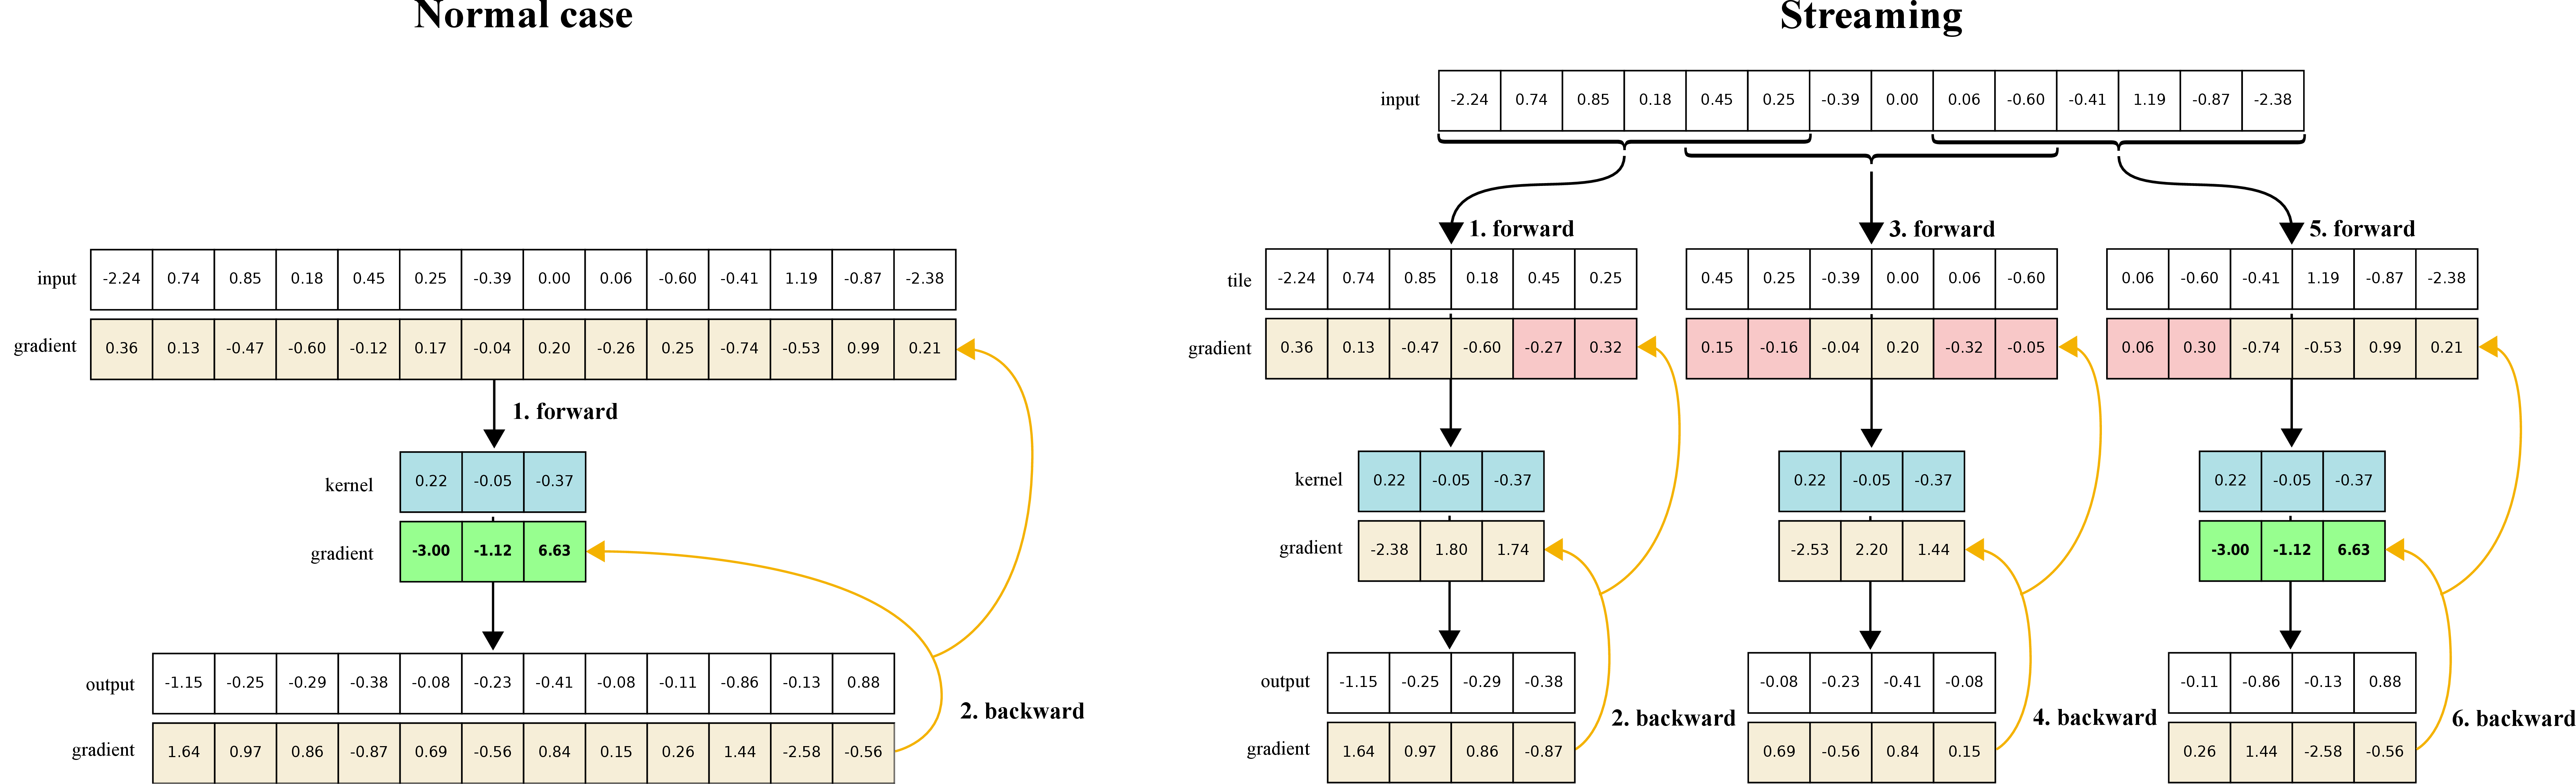
\includegraphics{chpt2_imgs/1dexample.png}

\hypertarget{calculateoverlap}{%
\subsection{Efficiently calculating required tile overlap for complex
architectures}\label{calculateoverlap}}

Some recent state-of-the-art networks (e.g., ResNet and DenseNet)
contain different paths through the network that sum or concatenate
activations from different layers together. These paths make it
difficult to manually calculate the required tile overlap for streaming.

To calculate the overlap for such networks, we temporarily replace all
convolutional kernel parameters with \(\frac{1}{n}\), where \(n\) was
the length of the kernel. This causes each entry in the convolutional
layer's output to be the average of the input image spanned by the
convolutional kernel. We then pass an all-ones tile through the network.
The required overlap will be the number of non-maximum values in the
activation maps and gradients at the border of the tiles, see Algorithm
\protect\hyperlink{algorithm:crop}{{[}algorithm:crop{]}}.

\(output\_stride\gets 1\) \(o\gets\)
\texttt{forward}\((layers[i..n], o)\) \(loss\gets\)
\texttt{criterion}\((o)\) \(g\gets\)
\texttt{backward}\((layers[n..i], loss)\)

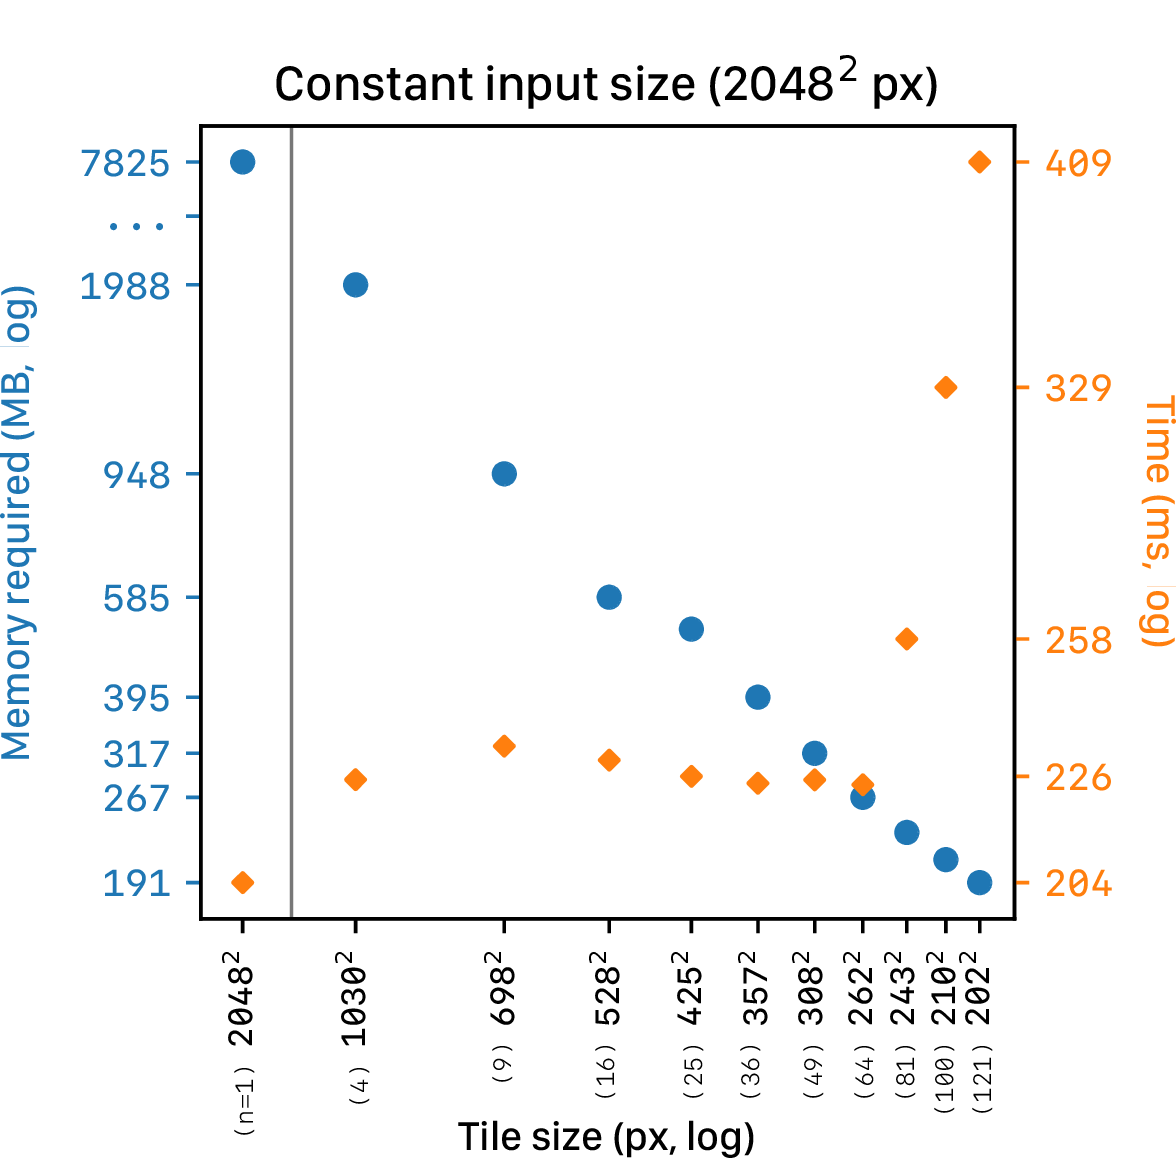
\includegraphics{chpt2_imgs/constant_input_size.png}\\

\hypertarget{limitations}{%
\subsection{Limitations}\label{limitations}}

With small tiles, the overlap can be a significant part of the tile,
counteracting the memory gains. Since we leverage the method for
high-resolution images using large tiles, the memory gains outweigh this
overhead.

Furthermore, due to the use of gradient checkpointing, the method will
perform multiple forward and backward operations to calculate
intermediate activations. This results in longer processing time than it
would take if the image could fit on the GPU (see Fig.
\protect\hyperlink{fig:constant_input}{{[}fig:constant\_input{]}} and
\protect\hyperlink{fig:constant_tile}{{[}fig:constant\_tile{]}}). The
processing time increases almost linearly with input size plus overlap.

For a network to be able to use this method, the intermediate feature
maps and its gradients have to be able to fit on the GPU at a certain
point. However, choosing a layer too deep into the network will require
a lot of overlapping calculations, being less efficient. As such,
choosing which layers to stream can be difficult. We suggest splitting
the network and experimenting with random input to the final
non-streaming layers to test if backpropagation fits on the GPU. Then,
streaming the first layers with a tile size as large as possible.

Finally, since the method relies on the local properties of convolutions
and pooling operations, trying to use other operations that break this
locality will result in invalid results (e.g., operations that rely on
all the feature map values such as
BatchNormalization\textsuperscript{31}). However, these operations can
be used as soon as the whole feature map is reconstructed, after
streaming, in the final part of the network.

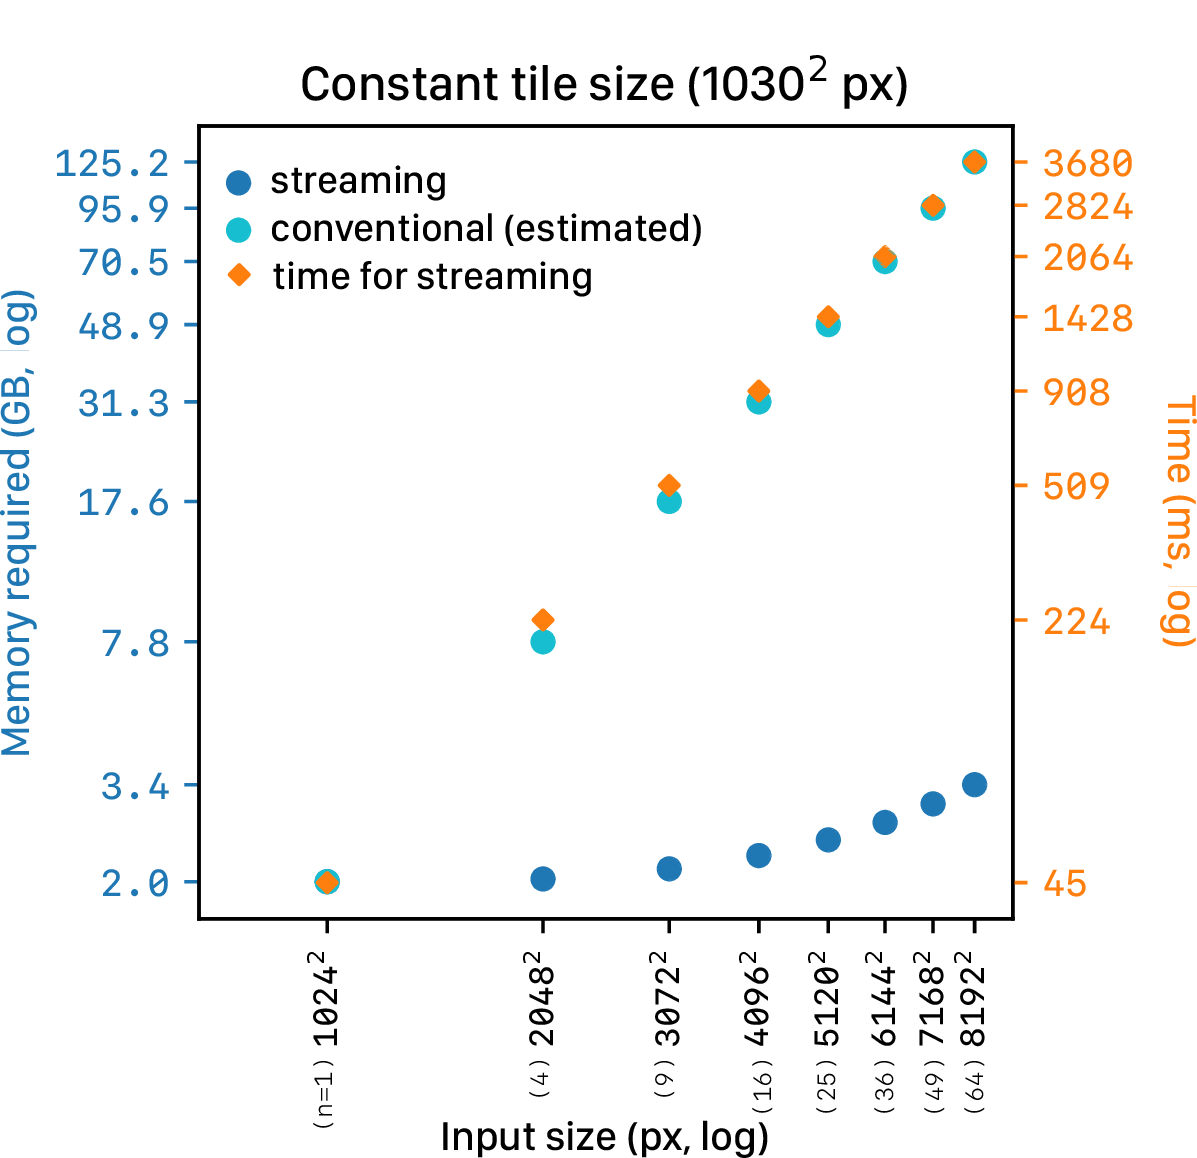
\includegraphics{chpt2_imgs/constant_tile_size.png}\\

\hypertarget{evaluation}{%
\section{Evaluation}\label{evaluation}}

We evaluated the streaming method with three different datasets and
network architectures. First, in Section
\protect\hyperlink{section:imagenette}{5}, we evaluated whether a CNN
using streaming trains equivalently to the conventional training.
Second, in Section \protect\hyperlink{section:tupac}{6}, we evaluated
the usage of streaming on a regression task in the public
TUPAC16\textsuperscript{9} dataset with high-resolution images (multiple
gigapixels) and only image-level labels. We trained multiple networks
using increasing image resolutions and network depth. Finally, in
Section \protect\hyperlink{section:camyleon}{7}, we evaluated streaming
in a classification task using the image-level labels of the CAMELYON17
dataset\textsuperscript{32}.

An open-source implementation of the streaming algorithm and the
ImageNette experiments can be found at
\url{https://github.com/DIAGNijmegen/StreamingCNN}.

\hypertarget{section:imagenette}{%
\section{Experiments on ImageNette}\label{section:imagenette}}

We trained a CNN on small images using streaming and conventional
training starting from the same initialization. We used a subset of the
ImageNet dataset, ImageNette, using 10 ImageNet classes (tench, English
springer, cassette player, chain saw, church, French horn, garbage
truck, gas pump, golf ball, parachute), analog to\textsuperscript{7}.

\hypertarget{tab:imagenetnet}{}
\begin{longtable}[]{@{}lll@{}}
\caption{Network architecture for Imagenette experiment}\tabularnewline
\toprule\noalign{}
\textbf{Layers} & \textbf{Kernel size} & \textbf{Channels} \\
\midrule\noalign{}
\endfirsthead
\toprule\noalign{}
\textbf{Layers} & \textbf{Kernel size} & \textbf{Channels} \\
\midrule\noalign{}
\endhead
\bottomrule\noalign{}
\endlastfoot
2D convolution & 3x3 & 16 \\
2D max-pool & 2x2 & 16 \\
2D convolution & 3x3 & 32 \\
2D max-pool & 2x2 & 32 \\
2D convolution & 3x3 & 64 \\
2D max-pool & 2x2 & 64 \\
2D convolution & 3x3 & 128 \\
2D max-pool & 2x2 & 128 \\
2D convolution & 3x3 & 256 \\
2D max-pool & 10x10 & 256 \\
Fully connected & 10 & \\
\end{longtable}

\hypertarget{data-preparation}{%
\subsection{Data preparation}\label{data-preparation}}

We used data augmentation for the training set following Szegedy et
al.\textsuperscript{33}. Patches of varying sizes were sampled from the
image, distributed evenly between 8\% and 100\% of the image area with
aspect ratio constrained to the interval \([\frac{3}{4}, \frac{4}{3}]\).
For the tuning set, we sampled 320\(\times\)320 patches from the center
of the image.

\hypertarget{network-architecture-and-training-scheme}{%
\subsection{Network architecture and training
scheme}\label{network-architecture-and-training-scheme}}

The CNN consisted of five blocks of a convolutional layer followed by a
max-pool layer (see Table \protect\hyperlink{tab:imagenetnet}{1}). The
network was optimized for 200 epochs with stochastic gradient descent,
using a learning rate of \(1 \times 10^{-3}\), a mini-batch size of 32
images and weight decay \(1 \times 10^{-6}\). For the streaming method,
the first four layers were streamed with tiles of 32\(\times\)32 pixels.
The network was initialized according to He et al.,
2015\textsuperscript{34}.

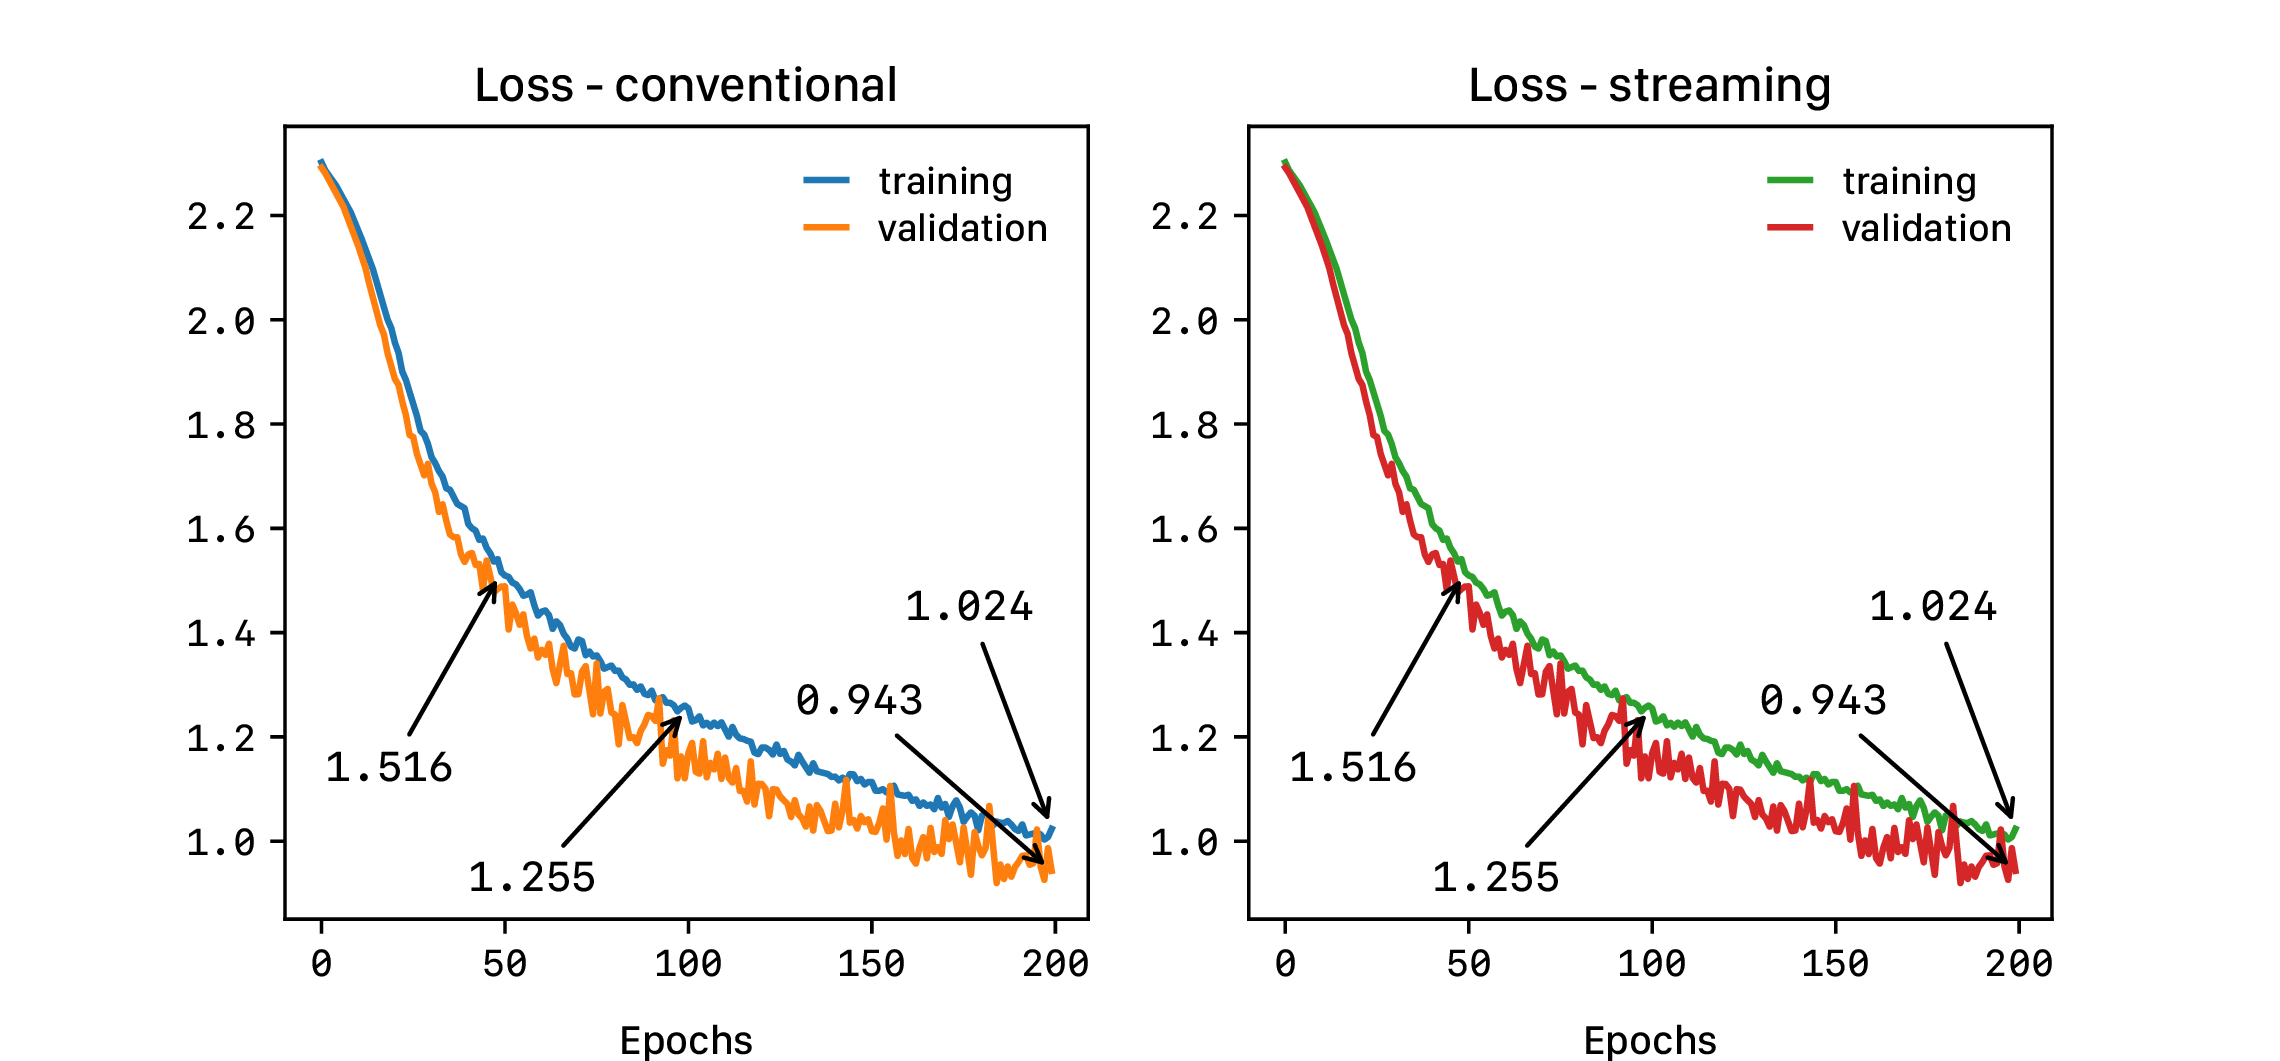
\includegraphics{chpt2_imgs/streamingvsnormal_rebuttal.png}\\
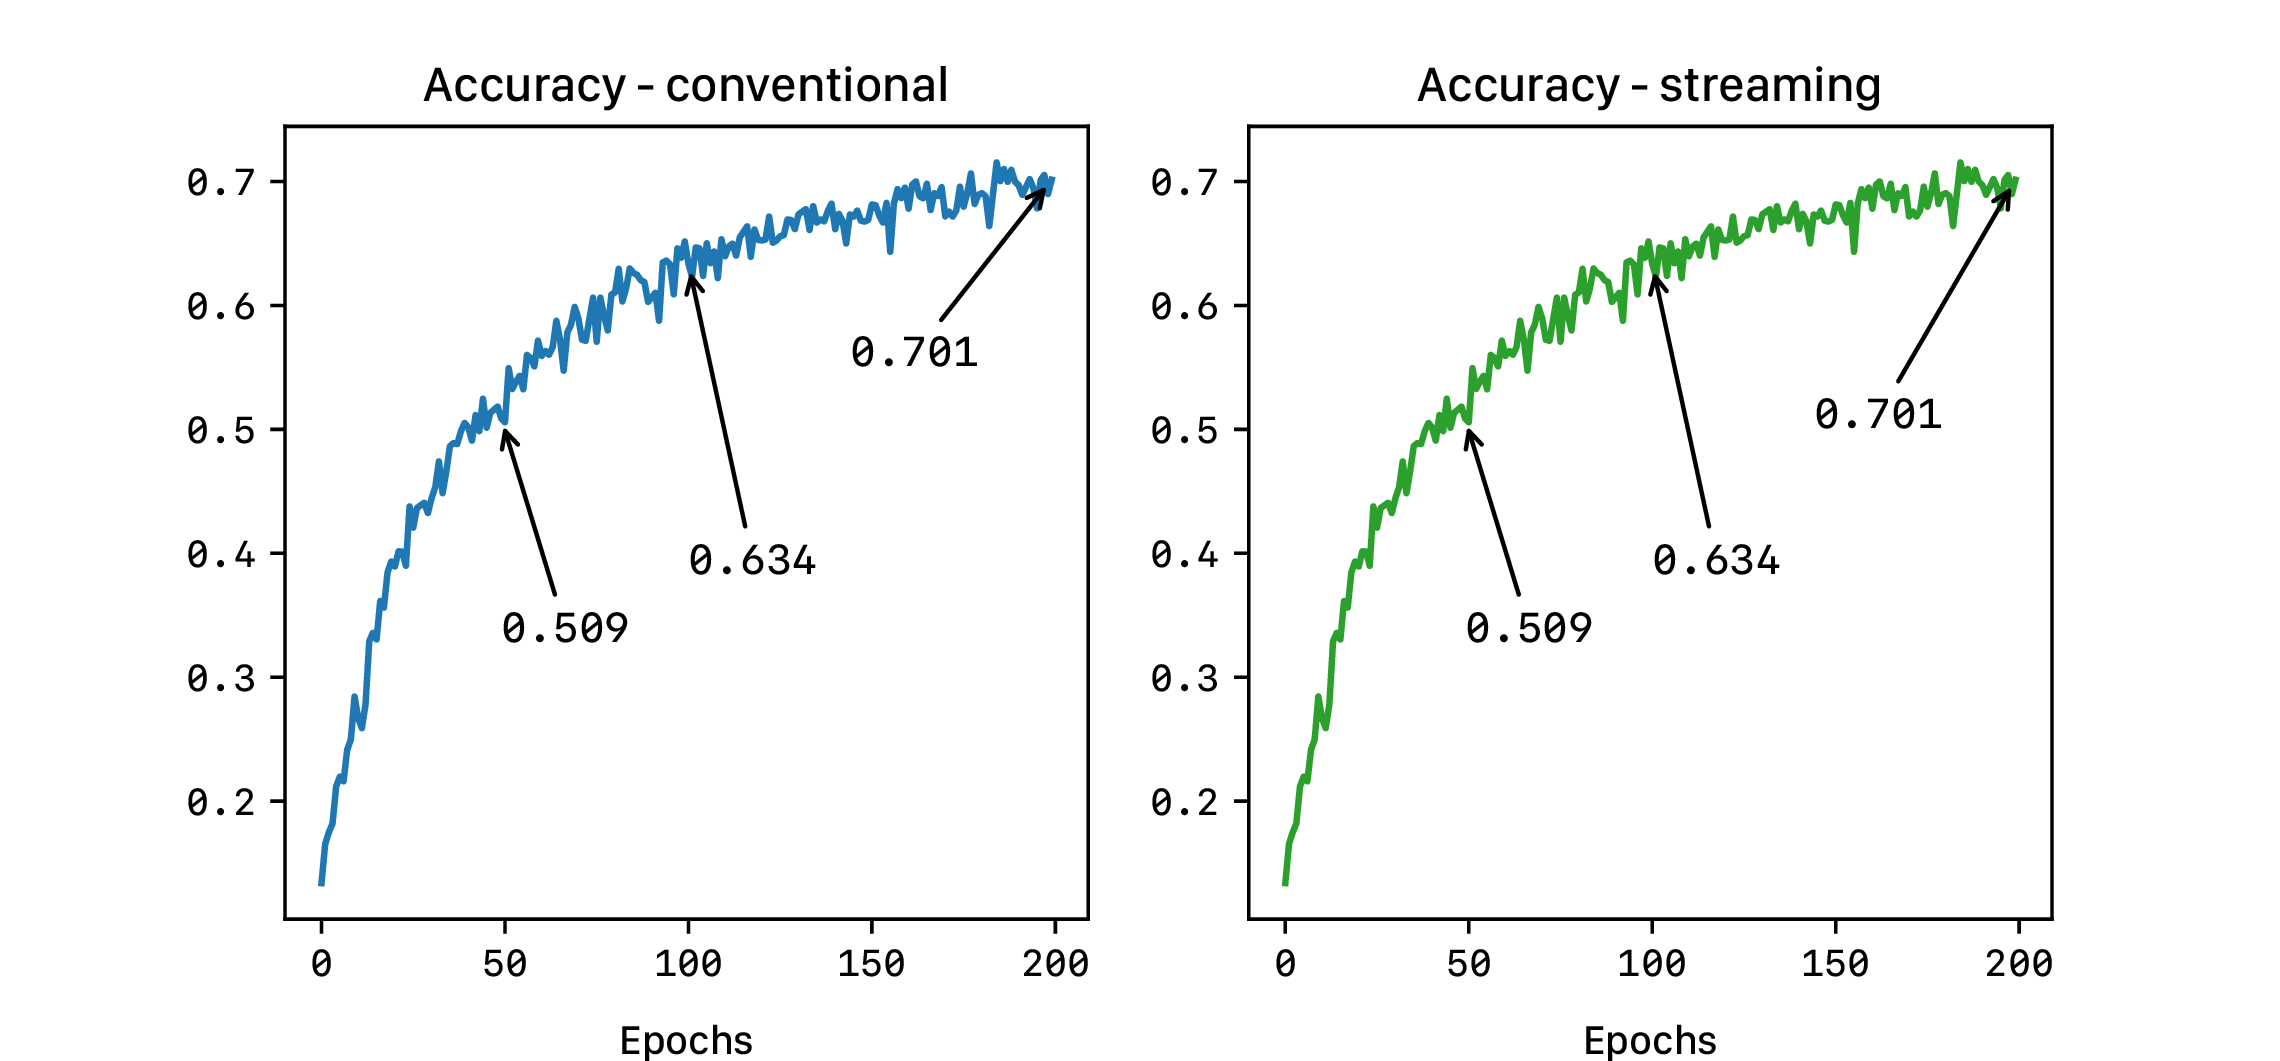
\includegraphics{chpt2_imgs/streamingvsnormal_accuracy_rebuttal.png}

\hypertarget{results-on-imagenette}{%
\subsection{Results on Imagenette}\label{results-on-imagenette}}

The loss curves of both methods (Figure
\protect\hyperlink{figure:imagenette_exp}{{[}figure:imagenette\_exp{]}})
were nearly identical, which empirically shows that training with
streaming performed equivalently to conventional training. Small
differences are likely due to losses of significance in floating point
arithmetic; these differences accumulate during training and lead to
small differences in loss values in later epochs.

\hypertarget{section:tupac}{%
\section{Experiments on TUPAC16 dataset}\label{section:tupac}}

To evaluate our method on a real-world task, we used the publicly
available dataset of the TUPAC16 challenge\textsuperscript{9}. This
dataset consists of 500 hematoxylin and eosin (H\&E) stained whole-slide
images (WSI) from breast adenocarcinoma patients. The WSIs of these
patients are available from The Cancer Genome Atlas\textsuperscript{35}
together with RNA expression profiles. The expression of 11
proliferation-associated genes was combined to create one objective
measure for tumor growth, termed the PAM50 score\textsuperscript{36}.
This score has no known visual substrate in the images. Thus, manual
labeling is considered impossible. We set aside 98 WSIs at random for
tuning the algorithm and used the remaining slides for training.
Additionally, an independent evaluation was performed by the challenge
organizers on the test set of 321 WSIs, of which the public ground truth
is not available. The submitted predictions were evaluated using
Spearman's rank-order correlation between the prediction and the ground
truth.

\hypertarget{tab:extset}{}
\begin{longtable}[]{@{}llll@{}}
\caption{Network architecture for TUPAC16 experiments.}\tabularnewline
\toprule\noalign{}
\endfirsthead
\endhead
\bottomrule\noalign{}
\endlastfoot
\textbf{Layers} & \textbf{Kernel} & \textbf{Channels} &
\textbf{Details} \\
2x 2D convolution & 3x3 & 32 & \\
2D max-pool & 2x2 & 32 & \\
2x 2D convolution & 3x3 & 64 & \\
2D max-pool & 2x2 & 64 & \\
2x 2D convolution & 3x3 & 128 & \\
2D max-pool & 2x2 & 128 & \\
2x 2D convolution & 3x3 & 256 & \\
2D max-pool & 2x2 & 256 & \\
2x 2D convolution & 3x3 & 512 & repeated for \\
2D max-pool & 2x2 & 512 & field of view experiment \\
2x 2D convolution & 3x3 & 512 & with BatchNormalization \\
2D max-pool & 2x2 & 512 & \\
2x 2D convolution & 3x3 & 512 & with BatchNormalization \\
2D max-pool & input size & 512 & \\
Dropout (p=0.5) & & 512 & \\
Fully connected & & & continuous output, \\
& & & without non-linearity \\
\end{longtable}

To evaluate whether CNN models can leverage and use the higher
resolution information that streaming makes possible, we performed two
sets of experiments to end-to-end predict the PAM50 score. For one, we
trained the same model with various image sizes (1024\(\times\)1024,
2048\(\times\)2048, and 4096\(\times\)4096 pixels), thus increasing
input image resolution. Different networks were trained in the second
set, where the depth was increased with image size (22, 25, and 28
layers for respectively 2048\(\times\)2048, 4096\(\times\)2096, and
8192\(\times\)8192). By also increasing the depth, the physical
receptive field size before the last max-pool layer is kept constant
(see Table \protect\hyperlink{tab:extset}{2}). All networks were trained
until convergence; the checkpoint with the highest Spearman's
correlation coefficient on the tuning set was submitted for independent
evaluation on the test set.

\hypertarget{data-preparation-1}{%
\subsection{Data preparation}\label{data-preparation-1}}

The images were extracted from the WSIs at image spacing \(16.0\mu m\)
for the 1024\(\times\)1024 experiments, \(8.0\mu m\) for
2048\(\times\)2048, etc. (see Figure
\protect\hyperlink{fig:resolutions}{{[}fig:resolutions{]}}). Background
regions were cropped, and the resulting image was either randomly
cropped or zero-padded to the predefined input size.

Since the challenge consists of a limited number of slides, we applied
extensive data augmentations to increase the sample size (random
rotations; random horizontal or vertical flipping; random brightness,
contrast, saturation, and hue shifts; elastic transformations; and
cutout\textsuperscript{37}). For all experiments, the same
hyperparameters and data preprocessing were used.

\hypertarget{network-architecture-and-training-scheme-1}{%
\subsection{Network architecture and training
scheme}\label{network-architecture-and-training-scheme-1}}

The networks (see Table \protect\hyperlink{tab:extset}{2}) were trained
using the Adam optimizer\textsuperscript{38} with a learning rate of
\(1 \times 10^{-4}\), with the default \(\beta\) parameters of
\(\beta_1=0.9\), \(\beta_2=0.999\). We applied exponential decay to the
learning rate of 0.99 per epoch. As an objective, we used the Huber loss
with \(\Delta=1\), also called the smooth L1 loss\textsuperscript{39}.
The mini-batch size was 16 images. A dropout layer with \(p=0.5\) was
inserted before the final classification layer. The networks were
initialized following He et al., 2015\textsuperscript{34}. The images
were normalized using the mean and standard deviation values of the
whole training set.

Streaming was applied until the final seven layers. Since
BatchNormalization breaks the local properties of chained convolutional
and pooling layers, it was only used in the last part of the network.
Analysis of Santurkar et al.\textsuperscript{40} suggests that adding
only a few BatchNormalization layers towards the end of the network
smooths the loss function significantly and helps optimization.

\hypertarget{results-on-tupac16}{%
\subsection{Results on TUPAC16}\label{results-on-tupac16}}

The task was evaluated using Spearman's correlation coefficient between
the prediction and the ground truth PAM50 proliferation scores. In both
experiments, an improvement of the metric was seen with increasing input
sizes.

\hypertarget{tab:tupacresults}{}
\begin{longtable}[]{@{}lll@{}}
\caption{TUPAC16: performance of the models on the independent test
test, Spearman's rho correlation coefficient}\tabularnewline
\toprule\noalign{}
\textbf{Experiment} & \textbf{Input size} & \textbf{Test set
performance} \\
\midrule\noalign{}
\endfirsthead
\toprule\noalign{}
\textbf{Experiment} & \textbf{Input size} & \textbf{Test set
performance} \\
\midrule\noalign{}
\endhead
\bottomrule\noalign{}
\endlastfoot
Equal number of parameters & 1024x1024 & 0.485 (0.441-0.527) \\
& 2048x2048 & 0.491 (0.448-0.533) \\
& 4096x4096 & 0.536 (0.495-0.575) \\
Equal field of view before global max-pool (increasing depth) &
2048x2048 & 0.491 (0.448-0.533) \\
& 4096x4096 & 0.570 (0.531-0.606) \\
& 8192x8192 & 0.560 (0.520-0.597) \\
\end{longtable}

The result of the network with the input image resolution of
4096\(\times\)4096 approached state-of-the-art for image-level
regression with a score of 0.570. Note that the first entry of the
leaderboard used an additional set of manual annotations of mitotic
figures and is therefore not directly comparable to our experiments.

\hypertarget{tab:tupacleaderboard}{}
\begin{longtable}[]{@{}ll@{}}
\caption{*method uses additional detailed annotations from another task
in the challenge and does not train a single model to predict from slide
to PAM50 score.}\tabularnewline
\toprule\noalign{}
\textbf{Experiment} & \textbf{Corr. coefficient} \\
\midrule\noalign{}
\endfirsthead
\toprule\noalign{}
\textbf{Experiment} & \textbf{Corr. coefficient} \\
\midrule\noalign{}
\endhead
\bottomrule\noalign{}
\endlastfoot
Lunit Inc., South Korea\textsuperscript{9,41} & 0.617* \\
\textbf{Ours (4096x4096)} & \textbf{0.570} \\
\textbf{Ours (8192x8192)} & \textbf{0.560} \\
Tellez et al., 2019\textsuperscript{23} & 0.557 \\
Radboud UMC Nijmegen, The Netherlands\textsuperscript{9} & 0.516 \\
Contextvision, Sweden\textsuperscript{9} & 0.503 \\
Belarus National Academy of Sciences\textsuperscript{9} & 0.494 \\
The Harker School, United States\textsuperscript{9} & 0.474 \\
\end{longtable}

\hypertarget{section:camyleon}{%
\section{Experiments on CAMELYON17 dataset}\label{section:camyleon}}

CAMELYON17 was used to evaluate the streaming method on a classification
task\textsuperscript{32}. CAMELYON17 is a large public dataset and
challenge to detect metastases of adenocarcinoma in breast tissue. The
dataset consists of 500 labelled WSIs and 500 unlabeled WSIs, which were
respectively used as the training and test sets. In the training set,
for 450 slides image-level labels were provided, while for the remaining
50 slides dense annotations (precise delineation of the metastases) were
supplied. The slides were collected from five different hospitals. The
challenge differentiates three clinical relevant metastases types:
macro-metastases (\(>\) 2 mm), micro-metastases (\(\leq\) 2.0 mm or
\(>\) 200 cells in a single cross-section), and isolated tumor cells
(\(\leq\) 0.2 mm or \(<\) 200 cells in a single cross-section). We
evaluate the slide level classification performance with multiple ROC
analyses (metastasis-type vs.~the negative class, and negative versus
all positive classes).

Data preparation for this experiment was equal to the TUPAC16 challenge.
We picked 90 WSIs of the challenge training set at random to be used as
our tuning set.

Confidence intervals were obtained through bootstrapping of the test
set, ensuring the same sampling across the different resolutions.
Furthermore, we performed a permutation test to assess statistical
significance.

\hypertarget{network-architecture-and-training-scheme-2}{%
\subsection{Network architecture and training
scheme}\label{network-architecture-and-training-scheme-2}}

We used the same training schedule and underlying architecture as the
TUPAC16 experiments. We altered the architecture by disabling dropout,
and to reduce problems with exploding gradients in the beginning of the
network, we replaced BatchNormalization with weight decay of
\(1 \times 10^{-6}\) and layer-sequential unit-variance (LSUV)
initialization\textsuperscript{42}. We applied the LSUV scaling per
kernel channel\textsuperscript{43}. The mean and standard deviation per
layer activation were calculated over ten mini-batches by keeping track
of the sum and squares of the channels per tile during streaming; the
reformulation of variance as \(\mathbb{E}[X^2] - \mu^2\) was used to
calculate the full standard deviation of ten mini-batches before
applying LSUV.

\begin{longtable}[]{@{}lllll@{}}
\toprule\noalign{}
\endhead
\bottomrule\noalign{}
\endlastfoot
\textbf{Input} & \textbf{Negative} & \textbf{Isolated tumor cells} &
\textbf{Micro-metastases} & \textbf{Macro-metastases} \\
& n=260 & n=35 & n=83 & n=122 \\
2048\(^2\) & 0.580 (0.529-0.628) & 0.450 (0.363-0.539) & 0.689
(0.620-0.755) & 0.515 (0.451-0.577) \\
4096\(^2\) & 0.648 (0.601-0.696, p\textsubscript{1}=0.03) &
\textbf{0.533} (0.422-0.642, p\textsubscript{1}=0.13) & 0.669
(0.602-0.733, p\textsubscript{1}=0.65) & 0.663 (0.603-0.719,
p\textsubscript{1}\textless0.001) \\
8192\(^2\) & \textbf{0.706} (0.660-0.751,
p\textsubscript{1}\textless0.001, p\textsubscript{2}=0.06) & 0.463
(0.359-0.569, p\textsubscript{1}=0.43, p\textsubscript{2}=0.83) &
\textbf{0.709} (0.645-0.769, p\textsubscript{1}=0.35,
p\textsubscript{2}=0.22) & \textbf{0.827} (0.777-0.874,
p\textsubscript{1}\textless0.001, p\textsubscript{2}\textless0.001) \\
\end{longtable}

\hypertarget{results-on-camelyon17}{%
\subsection{Results on CAMELYON17}\label{results-on-camelyon17}}

The network trained with 8192\(\times\)8192 images is significantly
better than the models trained with 4096\(\times\)4096 images in the
discriminating macro-metastases from negative cases, and significantly
better than the 2048\(\times\)2048 model in discriminating negative
cases from cases with any metastasis.

\hypertarget{saliency-maps}{%
\subsection{Saliency maps}\label{saliency-maps}}

Saliency maps were created for the networks trained with the largest
resolution (8192\(\times\)8192 pixels) according to Simonyan et
al.\textsuperscript{44}. For better visualization on lower resolution, a
Gaussian blur was applied with \(\sigma = 50\) for 8192\(\times\)8192
network, \(\sigma = 25\) for the 4096\(\times\)4096 models, and
\(\sigma = 12,5\) for the 2048\(\times\)2048 models. Since a few
gradient values can be significantly higher than others, we capped the
upper gradient values at the 99\textsuperscript{th}
percentile\textsuperscript{45}. The upper 50\textsuperscript{th}
percentile was overlayed on top of the original image (See Figure
\protect\hyperlink{figure:saliency}{2}).

\begin{figure}
\hypertarget{figure:saliency}{%
\centering
\includegraphics{chpt2_imgs/comparison_tupac.jpg}
\caption{Saliency maps for test set images of the TUPAC16 experiment
using the best performing models. The TUPAC16 network shows highlights
in cell-dense and cancerous regions. There is a trend in which the
higher the input solution of the model, the less it focuses on healthy
tissue. Also, higher resolution models focus on more locations of the
tissue.}\label{figure:saliency}
}
\end{figure}

\begin{figure}
\hypertarget{figure:saliency}{%
\centering
\includegraphics{chpt2_imgs/comparisoncam_rebuttal.jpg}
\caption{Saliency maps for images of the tuning set of the CAMELYON17
experiment. The highest resolution model, trained on image-level labels
shows highlights corresponding to the ground truth pixel-level
annotation of a breast cancer metastasis. The lower resolution models
have lower probability for the ground truth class and show little
correspondence to the location of the metastases. The last row shows a
micro metastasis for which models failed to
recognize.}\label{figure:saliency}
}
\end{figure}

\hypertarget{discussion-and-conclusion}{%
\section{Discussion and conclusion}\label{discussion-and-conclusion}}

We presented a novel streaming method to train CNNs with tiled inputs,
allowing inputs of arbitrary size. We showed that the reconstructed
gradients of the neural network weights using tiles were equivalent to
those obtained with non-tiled inputs.

In the first experiment on ImageNette, we empirically showed that the
training behavior of our proposed streaming method was similar to the
behavior in the non-streaming case. Small differences occur later in
training due to loss of significance in floating-point arithmetic. These
differences accumulated during training and lead to the small difference
in loss values in later epochs. However, they do not seem to harm
performance. Most modern frameworks have similar problems due to their
use of non-deterministic operations.

The second and third experiments showed that our streaming method can
train CNNs with multi-megapixel images that, due to memory requirements
in the non-streaming case, would not be able to fit on current hardware.
When trained using the conventional method, without streaming, the
experiment with the highest-resolution images (\(8192 \times 8192\)
pixels) would require \textasciitilde50 gigabytes per image, summing up
to \textasciitilde825 gigabytes of memory per mini-batch.

Results on the TUPAC16 dataset (Table
\protect\hyperlink{tab:tupacresults}{3}) showed an increasing
correlation between the prediction and the proliferation score with
increasing input sizes. Our 4096\(\times\)4096 pixel network performed
best. A jump in performance from 0.491 to 0.570 was seen from
2048\(\times\)2048 to 4096\(\times\)4096 pixels, respectively. We
hypothesize that this is because tumor tissue can be discriminated from
other types of tissue at these higher resolutions. However, an
8192\(\times\)8192 pixel input size did not further improve the
performance on the test set, although the difference is minor, and the
confidence interval is quite wide and overlapping. The nuclear details
of cells at this resolution remain vague, which suggests that most of
the information is still obtained from the morphology like in
4096\(\times\)4096 images. Higher resolutions may be necessary to
further improve performance, although we may also have hit the ceiling
for the performance of this network architecture, training setup, and
data. Another explanation for the lack of improvement is the increasing
difficulty for the network to find the sparse information in just 400
slides using a single label or a misrepresented tuning set due to the
small provided training set. As such, it is likely that for some tasks
and datasets, higher-resolutions are not beneficial. Our best result on
TUPAC16 approached that of the challenge winner, who used task-specific
information (a network trained on mitosis detection) instead of a pure
regression of one label per WSI. Our method outperformed all other
methods in the challenge.

Results on the CAMELYON17 dataset show improvement with increasing
resolution. An exception occurs for the isolated tumor cells class; even
at the highest resolution applied, the CNN was unable to differentiate
isolated tumor cells. To accurately identify lesions of that size, the
resolution would probably need to be increased by at least a factor of
four. Furthermore, this class is also underrepresented (n=31) in the
provided training set. The 8192\(\times\)8192 network was significantly
better than 4096\(\times\)4096 and 2048\(\times\)2048 in the
discriminating macro-metastases from negative cases and significantly
better than 2048\(\times\)2048 in discriminating negative cases from
cases with any metastasis.

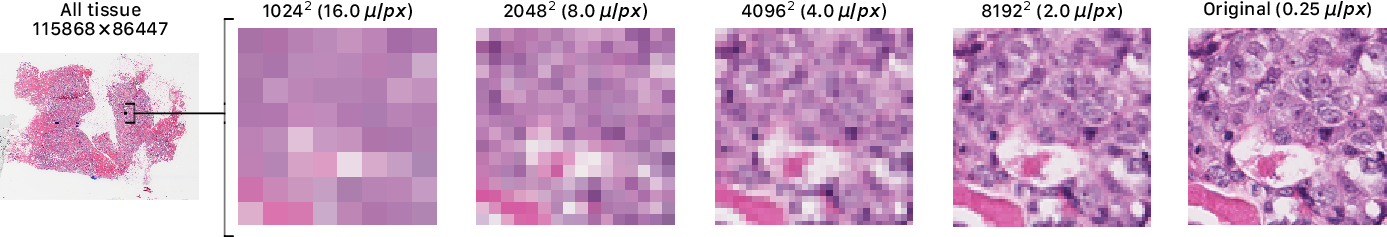
\includegraphics{chpt2_imgs/tupac_rebuttal.png}

Using saliency maps, we visualized what the models would change on the
input to make it more closely resemble the assigned class. These maps
show us which parts of the image the model takes into
consideration\textsuperscript{44}. Saliency maps of our CNNs trained on
higher resolutions suggest that the networks learn the relevant features
of the high-resolution images (see Figure
\protect\hyperlink{figure:saliency}{2}). The image-level trained
CAMELYON17 network shows highlights corresponding to the ground truth
pixel-level annotation of a breast cancer metastasis. The TUPAC16
network shows highlights in cell-dense regions.

The streaming method has advantages over prior work on this topic. For
streaming, we do not need to alter the dataset by resizing or creating
additional pixel-level labels (which is sometimes not possible). Also,
we do not need to change the usage of the dataset like in the MIL
paradigm or use compression techniques. Finally, we are not limited to
specific architectural choices for our network, such as in RevNet;
streaming can be applied to any state-of-the-art network, such as
Inception or DenseNet.

While increasing input sizes and resolutions are beneficial in various
tasks, there are some drawbacks. A limitation is the increase in
computation time with increasing input sizes (Fig.
\protect\hyperlink{fig:constant_tile}{{[}fig:constant\_tile{]}}). This
can be partially counteracted by dividing the batch over multiple GPUs.
Due to this limitation, we did not increase resolution further in our
experiments. Future research could attempt to speed up computation on
the tiles, e.g., by training with mixed precision\textsuperscript{29} or
depthwise separable convolutions\textsuperscript{25}. One could also try
to start with a pre-trained network (e.g., on ImageNet) and fine-tune
for a shorter period.

Another limitation is the inability to use feature map-wide operations
in the streaming part of the network, e.g., BatchNormalization. In this
work, we replaced some benefits of BatchNormalization, namely the
robustness against bad initialization and the regularization, with LSUV
initialization and weight decay. Future work could focus on
normalization techniques that retain the local properties of the
relation between the output and input of the streaming part of the
network, e.g., weight normalization\textsuperscript{46}.

Although this approach can, in theory, be used for segmentation,
streaming a segmentation network, such as U-Net\textsuperscript{47},
will require some engineering. We would have to stream the encoder,
"checkpointing" and reconstructing feature maps at the final convolution
of every level, for the skip connections. Then, we would have to stream
the decoding separately and carefully supply the spatially correct
regions of the checkpointed skip connections to each tile. Equally for
the backpropagation, reconstructing the gradients at the beginning of
each decode level to make the skip connections work. This would be the
case for a regular U-Net, if we would add more levels to U-Net, you will
have to train middle layers without streaming, as the field of view of
these layers could be too high (requiring a big overlap, making
streaming less memory efficient).

Improving the performance of the high-resolution-trained networks could
be a research topic of interest. In the TUPAC16 and CAMELYON17
experiments, we increased depth as we increased the input size. However,
a recent work\textsuperscript{26} -- though on a maximum
480\(\times\)480 image size -- suggests a ``compound'' scaling rule in
which the input resolution is scaled together with depth and width of
the network.

This paper focused on streaming two-dimensional images, but since
convolutions over higher-dimensional data have the same local
properties, one could leverage the same technique for, for example, 3D
volumetric radiological images.

\hypertarget{acknowledgements}{%
\section{Acknowledgements}\label{acknowledgements}}

The authors would like to thank Erdi Çallı~for his help in proofreading
the equations.

\hypertarget{refs}{}
\begin{CSLReferences}{0}{0}
\leavevmode\vadjust pre{\hypertarget{ref-Russakovsky2015}{}}%
\CSLLeftMargin{1. }%
\CSLRightInline{Russakovsky O, Deng J, Su H, et al. {ImageNet Large
Scale Visual Recognition Challenge}. \emph{International Journal of
Computer Vision}. 2015;115(3):211-252.
doi:\href{https://doi.org/10.1007/s11263-015-0816-y}{10.1007/s11263-015-0816-y}}

\leavevmode\vadjust pre{\hypertarget{ref-Krizhevsky2012}{}}%
\CSLLeftMargin{2. }%
\CSLRightInline{Krizhevsky A, Sutskever I, Hinton GE. {ImageNet
Classification with Deep Convolutional Neural Networks}. In:
\emph{Proceedings of the 25th Advances in Neural Information Processing
Systems}.; 2012.
\href{http://code.google.com/p/cuda-convnet/\%20http://papers.nips.cc/paper/4824-imagenet-classification-w\%5Cnpapers3://publication/uuid/1ECF396A-CEDA-45CD-9A9F-03344449DA2A}{http://code.google.com/p/cuda-convnet/
http://papers.nips.cc/paper/4824-imagenet-classification-w\%5Cnpapers3://publication/uuid/1ECF396A-CEDA-45CD-9A9F-03344449DA2A}}

\leavevmode\vadjust pre{\hypertarget{ref-He2016}{}}%
\CSLLeftMargin{3. }%
\CSLRightInline{He K, Zhang X, Ren S, Sun J. {Deep residual learning for
image recognition}. In: \emph{Proceedings of the IEEE Computer Society
Conference on Computer Vision and Pattern Recognition}. Vol 2016. IEEE
Computer Society; 2016:770-778.
doi:\href{https://doi.org/10.1109/CVPR.2016.90}{10.1109/CVPR.2016.90}}

\leavevmode\vadjust pre{\hypertarget{ref-Zagoruyko2016}{}}%
\CSLLeftMargin{4. }%
\CSLRightInline{Zagoruyko S, Komodakis N. {Wide Residual Networks}.
Published online May 2016. \url{http://arxiv.org/abs/1605.07146}}

\leavevmode\vadjust pre{\hypertarget{ref-Krizhevsky2009}{}}%
\CSLLeftMargin{5. }%
\CSLRightInline{Krizhevsky A. \emph{{Learning Multiple Layers of
Features from Tiny Images}}. University of Toronto; 2009.}

\leavevmode\vadjust pre{\hypertarget{ref-Chen2016a}{}}%
\CSLLeftMargin{6. }%
\CSLRightInline{Chen T, Xu B, Zhang C, Guestrin C. {Training Deep Nets
with Sublinear Memory Cost}. \emph{arXiv preprint}. 2016;1604.06174.
\url{http://arxiv.org/abs/1604.06174}}

\leavevmode\vadjust pre{\hypertarget{ref-Howard2019}{}}%
\CSLLeftMargin{7. }%
\CSLRightInline{Jeremy Howard. {Imagenette: a smaller subset of 10
easily classified classes from Imagenet, and a little more French}.
\url{https://github.com/fastai/imagenette}}

\leavevmode\vadjust pre{\hypertarget{ref-Litjens2018}{}}%
\CSLLeftMargin{8. }%
\CSLRightInline{Litjens G, Bandi P, Bejnordi BE, et al. {1399
H{\&}E-stained sentinel lymph node sections of breast cancer patients:
The CAMELYON dataset}. 2018;7.
doi:\href{https://doi.org/10.1093/gigascience/giy065}{10.1093/gigascience/giy065}}

\leavevmode\vadjust pre{\hypertarget{ref-Veta2019}{}}%
\CSLLeftMargin{9. }%
\CSLRightInline{Veta M, Heng YJ, Stathonikos N, et al. {Predicting
breast tumor proliferation from whole-slide images: The TUPAC16
challenge}. \emph{Medical Image Analysis}. 2019;54:111-121.
doi:\href{https://doi.org/10.1016/j.media.2019.02.012}{10.1016/j.media.2019.02.012}}

\leavevmode\vadjust pre{\hypertarget{ref-Ma2019}{}}%
\CSLLeftMargin{10. }%
\CSLRightInline{Ma L, Liu Y, Zhang X, Ye Y, Yin G, Johnson BA. {Deep
learning in remote sensing applications: A meta-analysis and review}.
2019;152:166-177.
doi:\href{https://doi.org/10.1016/j.isprsjprs.2019.04.015}{10.1016/j.isprsjprs.2019.04.015}}

\leavevmode\vadjust pre{\hypertarget{ref-Litjens2017}{}}%
\CSLLeftMargin{11. }%
\CSLRightInline{Litjens G, Kooi T, Bejnordi BE, et al. {A survey on deep
learning in medical image analysis}. 2017;42:60-88.
doi:\href{https://doi.org/10.1016/j.media.2017.07.005}{10.1016/j.media.2017.07.005}}

\leavevmode\vadjust pre{\hypertarget{ref-Campanella2019}{}}%
\CSLLeftMargin{12. }%
\CSLRightInline{Campanella G, Hanna MG, Geneslaw L, et al.
{Clinical-grade computational pathology using weakly supervised deep
learning on whole slide images}. \emph{Nature Medicine}.
2019;25(8):1301-1309.
doi:\href{https://doi.org/10.1038/s41591-019-0508-1}{10.1038/s41591-019-0508-1}}

\leavevmode\vadjust pre{\hypertarget{ref-Courtiol2018}{}}%
\CSLLeftMargin{13. }%
\CSLRightInline{Courtiol P, Tramel EW, Sanselme M, Wainrib G.
{Classification and Disease Localization in Histopathology Using Only
Global Labels: A Weakly-Supervised Approach}. \emph{arXiv preprint}.
2018;1802.02212. \url{http://arxiv.org/abs/1802.02212}}

\leavevmode\vadjust pre{\hypertarget{ref-Quellec2017}{}}%
\CSLLeftMargin{14. }%
\CSLRightInline{Quellec G, Cazuguel G, Cochener B, Lamard M.
{Multiple-Instance Learning for Medical Image and Video Analysis}.
\emph{IEEE Reviews in Biomedical Engineering}. 2017;10:213-234.
doi:\href{https://doi.org/10.1109/RBME.2017.2651164}{10.1109/RBME.2017.2651164}}

\leavevmode\vadjust pre{\hypertarget{ref-Ilse2018}{}}%
\CSLLeftMargin{15. }%
\CSLRightInline{Ilse M, Tomczak JM, Welling M. {Attention-based Deep
Multiple Instance Learning}. \emph{arXiv preprint}. 2018;1802.04712.
\url{http://arxiv.org/abs/1802.04712}}

\leavevmode\vadjust pre{\hypertarget{ref-Couture2018}{}}%
\CSLLeftMargin{16. }%
\CSLRightInline{Couture HD, Marron JS, Perou CM, Troester MA, Niethammer
M. {Multiple Instance Learning for Heterogeneous Images: Training a CNN
for Histopathology}. In: Frangi AF, Schnabel JA, Davatzikos C,
Alberola-López C, Fichtinger G, eds. \emph{Medical Image Computing and
Computer Assisted Intervention -- MICCAI 2018}. Springer International
Publishing; 2018:254-262.}

\leavevmode\vadjust pre{\hypertarget{ref-Ianni2020}{}}%
\CSLLeftMargin{17. }%
\CSLRightInline{Ianni JD, Soans RE, Sankarapandian S, et al. {Tailored
for Real-World: A Whole Slide Image Classification System Validated on
Uncurated Multi-Site Data Emulating the Prospective Pathology Workload}.
\emph{Scientific Reports}. 2020;10(1):3217.
doi:\href{https://doi.org/10.1038/s41598-020-59985-2}{10.1038/s41598-020-59985-2}}

\leavevmode\vadjust pre{\hypertarget{ref-Hou2016}{}}%
\CSLLeftMargin{18. }%
\CSLRightInline{Hou L, Samaras D, Kurc TM, Gao Y, Davis JE, Saltz JH.
{Patch-Based Convolutional Neural Network for Whole Slide Tissue Image
Classification}. In: \emph{2016 IEEE Conference on Computer Vision and
Pattern Recognition (CVPR)}.; 2016:2424-2433.
doi:\href{https://doi.org/10.1109/CVPR.2016.266}{10.1109/CVPR.2016.266}}

\leavevmode\vadjust pre{\hypertarget{ref-Dong2018}{}}%
\CSLLeftMargin{19. }%
\CSLRightInline{Dong N, Kampffmeyer M, Liang X, Wang Z, Dai W, Xing EP.
{Reinforced Auto-Zoom Net: Towards Accurate and Fast Breast Cancer
Segmentation in Whole-slide Images}. \emph{CoRR}. 2018;abs/1807.1.
\url{http://arxiv.org/abs/1807.11113}}

\leavevmode\vadjust pre{\hypertarget{ref-Mnih2014}{}}%
\CSLLeftMargin{20. }%
\CSLRightInline{Mnih V, Heess N, Graves A, Kavukcuoglu K. {Recurrent
Models of Visual Attention}. In: \emph{Proceedings of the 27th
International Conference on Neural Information Processing Systems -
Volume 2}. MIT Press; 2014:2204-2212.
\url{http://dl.acm.org/citation.cfm?id=2969033.2969073}}

\leavevmode\vadjust pre{\hypertarget{ref-Katharopoulos2019}{}}%
\CSLLeftMargin{21. }%
\CSLRightInline{Katharopoulos A, Fleuret F. {Processing Megapixel Images
with Deep Attention-Sampling Models}. In: \emph{Proceedings of the 36th
International Conference on Machine Learning}.; 2019.
\url{http://arxiv.org/abs/1905.03711}}

\leavevmode\vadjust pre{\hypertarget{ref-Recasens2018}{}}%
\CSLLeftMargin{22. }%
\CSLRightInline{Recasens A, Kellnhofer P, Stent S, Matusik W, Torralba
A. {Learning to Zoom: a Saliency-Based Sampling Layer for Neural
Networks}. In: \emph{European Conference on Computer Vision}.; 2018.
\url{http://arxiv.org/abs/1809.03355}}

\leavevmode\vadjust pre{\hypertarget{ref-Tellez2019}{}}%
\CSLLeftMargin{23. }%
\CSLRightInline{Tellez D, Litjens G, Laak J van der, Ciompi F. {Neural
Image Compression for Gigapixel Histopathology Image Analysis}.
\emph{IEEE Transactions on Pattern Analysis and Machine Intelligence}.
in press.
doi:\href{https://doi.org/10.1109/TPAMI.2019.2936841}{10.1109/TPAMI.2019.2936841}}

\leavevmode\vadjust pre{\hypertarget{ref-Gomez2017}{}}%
\CSLLeftMargin{24. }%
\CSLRightInline{Gomez AN, Ren M, Urtasun R, Grosse RB. {The Reversible
Residual Network: Backpropagation Without Storing Activations}. In:
\emph{Proceedings of the 31st International Conference on Neural
Information Processing Systems}.; 2017:2211-2221.
\url{http://arxiv.org/abs/1707.04585}}

\leavevmode\vadjust pre{\hypertarget{ref-Chollet2017}{}}%
\CSLLeftMargin{25. }%
\CSLRightInline{Chollet F. {Xception: Deep Learning with Depthwise
Separable Convolutions}. In: \emph{2017 IEEE Conference on Computer
Vision and Pattern Recognition (CVPR)}.; 2017:1800-1807.
doi:\href{https://doi.org/10.1109/CVPR.2017.195}{10.1109/CVPR.2017.195}}

\leavevmode\vadjust pre{\hypertarget{ref-Tan2019}{}}%
\CSLLeftMargin{26. }%
\CSLRightInline{Tan M, Le QV. {EfficientNet: Rethinking Model Scaling
for Convolutional Neural Networks}. In: \emph{Proceedings of the 36th
International Conference on Machine Learning}.; 2019.
\url{http://arxiv.org/abs/1905.11946}}

\leavevmode\vadjust pre{\hypertarget{ref-Huang2017}{}}%
\CSLLeftMargin{27. }%
\CSLRightInline{Huang G, Liu Z, Van Der Maaten L, Weinberger KQ.
{Densely connected convolutional networks}. In: \emph{Proceedings - 30th
IEEE Conference on Computer Vision and Pattern Recognition}. Institute
of Electrical; Electronics Engineers Inc.; 2017:2261-2269.
doi:\href{https://doi.org/10.1109/CVPR.2017.243}{10.1109/CVPR.2017.243}}

\leavevmode\vadjust pre{\hypertarget{ref-Bulo2018}{}}%
\CSLLeftMargin{28. }%
\CSLRightInline{Bulo SR, Porzi L, Kontschieder P. {In-place Activated
BatchNorm for Memory-Optimized Training of DNNs}. In: \emph{Proceedings
of the IEEE Computer Society Conference on Computer Vision and Pattern
Recognition}.; 2018.
doi:\href{https://doi.org/10.1109/CVPR.2018.00591}{10.1109/CVPR.2018.00591}}

\leavevmode\vadjust pre{\hypertarget{ref-Vanhoucke2011}{}}%
\CSLLeftMargin{29. }%
\CSLRightInline{Vanhoucke V, Senior A, Mao MZ. {Improving the speed of
neural networks on CPUs}. In: \emph{Deep Learning and Unsupervised
Feature Learning Workshop, NIPS 2011}.; 2011.}

\leavevmode\vadjust pre{\hypertarget{ref-Zhang2019}{}}%
\CSLLeftMargin{30. }%
\CSLRightInline{Zhang J, Yeung SH, Shu Y, He B, Wang W. {Efficient
Memory Management for GPU-based Deep Learning Systems}. Published online
February 2019. \url{http://arxiv.org/abs/1903.06631}}

\leavevmode\vadjust pre{\hypertarget{ref-Ioffe2015}{}}%
\CSLLeftMargin{31. }%
\CSLRightInline{Ioffe S, Szegedy C. {Batch Normalization: Accelerating
Deep Network Training by Reducing Internal Covariate Shift}. In:
\emph{Proceedings of the 32Nd International Conference on International
Conference on Machine Learning - Volume 37}. ICML'15. JMLR.org;
2015:448-456. \url{http://dl.acm.org/citation.cfm?id=3045118.3045167}}

\leavevmode\vadjust pre{\hypertarget{ref-Bandi2019}{}}%
\CSLLeftMargin{32. }%
\CSLRightInline{Bándi P, Geessink O, Manson Q, et al. {From Detection of
Individual Metastases to Classification of Lymph Node Status at the
Patient Level: The CAMELYON17 Challenge}. \emph{IEEE Transactions on
Medical Imaging}. 2019;38(2):550-560.
doi:\href{https://doi.org/10.1109/TMI.2018.2867350}{10.1109/TMI.2018.2867350}}

\leavevmode\vadjust pre{\hypertarget{ref-Szegedy2015}{}}%
\CSLLeftMargin{33. }%
\CSLRightInline{Szegedy C, Wei Liu, Yangqing Jia, et al. {Going deeper
with convolutions}. In: \emph{2015 IEEE Conference on Computer Vision
and Pattern Recognition (CVPR)}.; 2015:1-9.
doi:\href{https://doi.org/10.1109/CVPR.2015.7298594}{10.1109/CVPR.2015.7298594}}

\leavevmode\vadjust pre{\hypertarget{ref-He:2015:DDR:2919332.2919814}{}}%
\CSLLeftMargin{34. }%
\CSLRightInline{He K, Zhang X, Ren S, Sun J. {Delving Deep into
Rectifiers: Surpassing Human-Level Performance on ImageNet
Classification}. In: \emph{Proceedings of the 2015 IEEE International
Conference on Computer Vision (ICCV)}. IEEE Computer Society;
2015:1026-1034.
doi:\href{https://doi.org/10.1109/ICCV.2015.123}{10.1109/ICCV.2015.123}}

\leavevmode\vadjust pre{\hypertarget{ref-Weinstein2013}{}}%
\CSLLeftMargin{35. }%
\CSLRightInline{Weinstein JN, Collisson EA, Mills GB, et al. {The Cancer
Genome Atlas Pan-Cancer analysis project}. \emph{Nature Genetics}.
2013;45(10):1113-1120.
doi:\href{https://doi.org/10.1038/ng.2764}{10.1038/ng.2764}}

\leavevmode\vadjust pre{\hypertarget{ref-Nielsen2010}{}}%
\CSLLeftMargin{36. }%
\CSLRightInline{Nielsen TO, Parker JS, Leung S, et al. {A Comparison of
PAM50 Intrinsic Subtyping with Immunohistochemistry and Clinical
Prognostic Factors in Tamoxifen-Treated Estrogen Receptor--Positive
Breast Cancer}. \emph{Clinical Cancer Research}. 2010;16(21):5222-5232.
doi:\href{https://doi.org/10.1158/1078-0432.CCR-10-1282}{10.1158/1078-0432.CCR-10-1282}}

\leavevmode\vadjust pre{\hypertarget{ref-DeVries2017}{}}%
\CSLLeftMargin{37. }%
\CSLRightInline{DeVries T, Taylor GW. {Improved Regularization of
Convolutional Neural Networks with Cutout}. \emph{CoRR}.
2017;abs/1708.0. \url{http://arxiv.org/abs/1708.04552}}

\leavevmode\vadjust pre{\hypertarget{ref-Kingma2015}{}}%
\CSLLeftMargin{38. }%
\CSLRightInline{Kingma DP, Ba J. {Adam: A method for stochastic
optimization}. In: \emph{International Conference on Learning
Representations (ICLR)}.; 2015.}

\leavevmode\vadjust pre{\hypertarget{ref-Girshick:2015:FR:2919332.2920125}{}}%
\CSLLeftMargin{39. }%
\CSLRightInline{Girshick R. {Fast R-CNN}. In: \emph{Proceedings of the
2015 IEEE International Conference on Computer Vision (ICCV)}. ICCV '15.
IEEE Computer Society; 2015:1440-1448.
doi:\href{https://doi.org/10.1109/ICCV.2015.169}{10.1109/ICCV.2015.169}}

\leavevmode\vadjust pre{\hypertarget{ref-Santurkar2018}{}}%
\CSLLeftMargin{40. }%
\CSLRightInline{Santurkar S, Tsipras D, Ilyas A, Madry A. {How does
batch normalization help optimization?} In: \emph{Advances in Neural
Information Processing Systems}. Vol 2018-Decem.; 2018:2483-2493.
\url{https://papers.nips.cc/paper/7515-how-does-batch-normalization-help-optimization.pdf}}

\leavevmode\vadjust pre{\hypertarget{ref-Paeng2016}{}}%
\CSLLeftMargin{41. }%
\CSLRightInline{Paeng K, Hwang S, Park S, Kim M. {A Unified Framework
for Tumor Proliferation Score Prediction in Breast Histopathology}.
\emph{CoRR}. 2016;abs/1612.0. \url{http://arxiv.org/abs/1612.07180}}

\leavevmode\vadjust pre{\hypertarget{ref-Mishkin2015}{}}%
\CSLLeftMargin{42. }%
\CSLRightInline{Mishkin D, Matas J. {All you need is a good init}. In:
\emph{International Conference on Learning Representations (ICLR)}.;
2016. \url{http://arxiv.org/abs/1511.06422}}

\leavevmode\vadjust pre{\hypertarget{ref-Krahenbuhl2015}{}}%
\CSLLeftMargin{43. }%
\CSLRightInline{Krähenbühl P, Doersch C, Donahue J, Darrell T.
{Data-dependent Initializations of Convolutional Neural Networks}. In:
\emph{International Conference on Learning Representations (ICLR)}.;
2016. \url{http://arxiv.org/abs/1511.06856}}

\leavevmode\vadjust pre{\hypertarget{ref-Simonyan2013}{}}%
\CSLLeftMargin{44. }%
\CSLRightInline{Simonyan K, Vedaldi A, Zisserman A. {Deep Inside
Convolutional Networks: Visualising Image Classification Models and
Saliency Maps}. \emph{CoRR}. Published online December 2013.
\url{http://arxiv.org/abs/1312.6034}}

\leavevmode\vadjust pre{\hypertarget{ref-Smilkov2017}{}}%
\CSLLeftMargin{45. }%
\CSLRightInline{Smilkov D, Thorat N, Kim B, Viégas FB, Wattenberg M.
{SmoothGrad: removing noise by adding noise}. In: \emph{ICML Workshop on
Visualization for Deep Learning}.; 2017.
\url{http://arxiv.org/abs/1706.03825}}

\leavevmode\vadjust pre{\hypertarget{ref-Salimans2016}{}}%
\CSLLeftMargin{46. }%
\CSLRightInline{Salimans T, Kingma DP. {Weight normalization: A simple
reparameterization to accelerate training of deep neural networks}. In:
\emph{Advances in Neural Information Processing Systems}.; 2016.}

\leavevmode\vadjust pre{\hypertarget{ref-ronneberger2015u}{}}%
\CSLLeftMargin{47. }%
\CSLRightInline{Ronneberger O, Fischer P, Brox T. {U-net: Convolutional
networks for biomedical image segmentation}. In: \emph{International
Conference on Medical Image Computing and Computer-Assisted
Intervention}. Springer; 2015:234-241.}

\end{CSLReferences}

\end{document}
